% Pressure-scope revision: analyses/021-2026-09-10-training-results-figures/pressure-scope/observations/O016-pressure-placement.md; evidence.py, figures.py, tables.py.
% Experimental setup/comparison logic and the user-authorized kernel case study.
% Provenance and scope: experimental-notes.md.
\section{Experimental study}
\label{sec:experiments}

We pretrain Pythia-14M, 70M, and 410M from random initialization~\citep{biderman2023pythia} on MiniPile~\citep{kaddour2023minipile}, using 1.493 billion input tokens per model. We evaluate validation loss and $\Smodel$ over all complete validation sequences. Table~\ref{tab:interventions} defines the thresholding and OL1-pressure recipes and their sparsity ceilings.

\textbf{Roles of the three scales.}
The 14M controlled intervention study identifies threshold- and pressure-placement
regimes. The 70M targeted replication tests whether those regimes recur.
The 410M fixed-token stress test examines attainable sparsity in a larger
architecture, not language-model quality scaling. All models receive the same
712 optimizer steps; the resulting tokens per parameter and the 410M
learning-rate schedule differ (Appendix~\ref{app:training-protocol}).

% 70M extension: runs/034-2026-09-17-pythia70m-h-only-ol1/README.md;
% Figure 1 evidence: Analysis024 observations/025-matched-quality-latency.md.
Within each size, runs share initialization, data order and training budget.
Appendix~\ref{app:training-protocol} gives the full protocol.
For comparison, we apply TEAL-style post-hoc magnitude thresholding~\citep{liu2024teal}
at $a,m,h,z$, with percentile targets $p=0,0.1,\ldots,0.9$ and site--layer
thresholds calibrated separately on ten training blocks.

% Recipe source: manuscript/artifacts/sparsification-ladder.tex and .md.
% Exact ceiling counts: reviews/2026-09-05-methodology/ceiling-verification.json.
\begin{table}[!htbp]
\centering\small
\caption{\textbf{Thresholding, pressure and sparsity ceilings.}
$T_1$ replaces GeLU with ReLU at $h$. Pressure uses OL1: $P_1=P_h$ targets
$h$, and $P_{\mathrm{all}}$ matches the thresholding sites
($\mathcal{P}=\mathcal{N}$). For $T_4/T_7$, threshold strength is swept over
$\kappa\in\{0,0.01,0.05,0.1,0.5\}$, with OL1 pressure weight $\lambda=1$
and task-relative norm budget $b=1$ fixed. OL1 limits conflict with the
adaptive task direction and uses the full allowed norm when its cap binds
(Appendix~\ref{app:pressure}), motivating a shared setting without a
loss-preservation guarantee. The 14M $T_1/P_1$ ablation instead sweeps
$\lambda\in\{0.05,0.1,0.5,1\}$ at $b=1$.
Ceilings are $100\cdot\Smax$ at 2,048 tokens; executed recipes by model size
are listed in Appendix~\ref{app:training-protocol}.}
\label{tab:interventions}
\vspace{4pt}
\setlength{\tabcolsep}{5pt}
\begin{tabular}{@{}lllrrr@{}}
\toprule
Recipe & Threshold sites $\mathcal{N}$ & Pressure sites $\mathcal{P}$ & \multicolumn{3}{c}{Ceiling (\%)} \\
\cmidrule(l){4-6}
 & & & 14M & 70M & 410M \\
\midrule
$T_0/P_0$ (Base Model) & $\varnothing$ & $\varnothing$ & 0.00 & 0.00 & 0.00 \\
\midrule
$T_1/P_0$ & $h$ & $\varnothing$ & 4.28 & 12.35 & 24.93 \\
$T_1/P_1$ & $h$ & $h$ & 4.28 & 12.35 & 24.93 \\
\midrule
$T_4/P_0$ & $a,m,h,z$ & $\varnothing$ & 12.83 & 37.06 & 74.78 \\
$T_4/P_h$ & $a,m,h,z$ & $h$ & 12.83 & 37.06 & 74.78 \\
$T_4/P_{\mathrm{all}}$ & $a,m,h,z$ & $\mathcal{N}$ & 12.83 & 37.06 & 74.78 \\
\midrule
$T_7/P_0$ & $a,m,h,z,q,k,v$ & $\varnothing$ & 29.95 & 49.42 & 87.25 \\
$T_7/P_h$ & $a,m,h,z,q,k,v$ & $h$ & 29.95 & 49.42 & 87.25 \\
$T_7/P_{\mathrm{all}}$ & $a,m,h,z,q,k,v$ & $\mathcal{N}$ & 29.95 & 49.42 & 87.25 \\
\bottomrule
\end{tabular}
\end{table}

\FloatBarrier
% Review corrections: Analysis 021 observations/O015-review-corrections.md; 10_review_figures.py.
\subsection{Quality--sparsity trade-offs}
\label{sec:quality-sparsity-results}

Local pressure and broader thresholds offer different trade-offs
(Figure~\ref{fig:quality-sparsity-overview}). One-site ReLU + OL1 at
$\lambda=0.5$ reaches $3.768\%$ sparsity and loss 5.1102, versus dense
loss 5.2086. Post-hoc magnitude thresholding of the dense reference reaches
similar sparsity, $3.832\%$, at loss 5.3619. Broader trained recipes reach
larger $\Smodel$, but seven-site placement also has more computational reach
than the four-site post-hoc comparator: $29.952\%$ versus $12.833\%$ at
14M. Thus the broad comparison changes both learned representation and
reachable computation; it does not establish universal dominance over
matched-site post-hoc methods. One-site OL1 is also not uniformly better
than naive L1: their small loss differences reverse at $\lambda=1$
(Appendix Table~\ref{tab:paired-effects-full}).

\subsection{Paired effect of adding pressure}
\label{sec:paired-results}

We compare pressure-on and pressure-free recipes at each matched $\kappa$
(Figure~\ref{fig:paired-intervention-effects}). Four-site OL1 slightly
improves loss at $\kappa=0$ and $0.01$, adding $0.598$ and $1.173$ pp of
$\Smodel$. Its increment reaches $2.498$ pp for $+0.3783$ loss at
$\kappa=0.5$. Seven-site OL1 adds $1.372$ pp for $+0.0008$ loss at
$\kappa=0.1$, but $12.096$ pp for $+0.1265$ at $0.5$.
\textbf{Pressure's marginal benefit depends on both threshold and target set.}

Define the complete-recipe interaction
$I_S(\kappa)=(S_{7,+}-S_{7,-})-(S_{4,+}-S_{4,-})$, where $+$ and $-$ denote
OL1 and no pressure; define $I_L$ analogously for loss. At $\kappa=0.5$,
$I_S=+9.598$ pp and $I_L=-0.2518$. Expanding to seven sites changes both
pressure targets and their equal-tensor normalization, so this is not an
isolated effect of Q/K/V pressure. The large difference occurs at the
largest sampled threshold; the gap from 0.1 to 0.5 does not identify a
transition or its location.

\begin{figure}[!t]
\centering
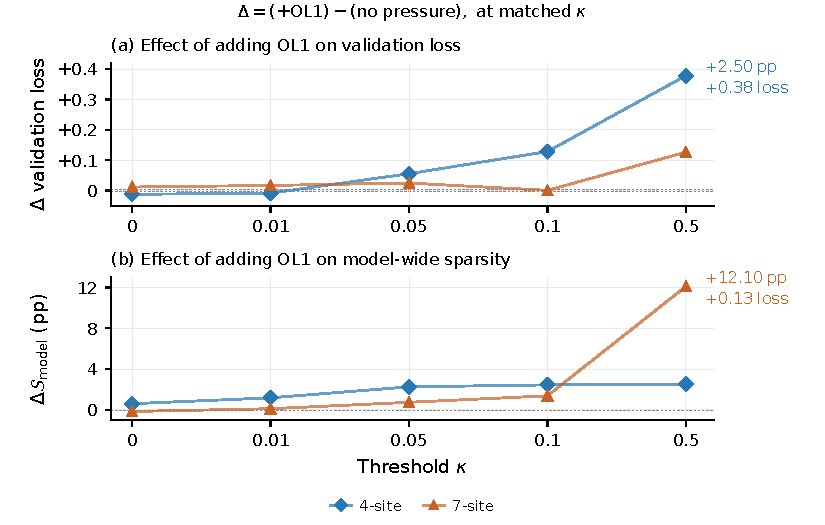
\includegraphics[width=.88\linewidth]{figures/03-14m-paired-interventions.pdf}
\caption{\textbf{Conditional effects of adding OL1.} Each point subtracts
the pressure-free endpoint from its OL1 counterpart at the same trained
$\kappa$: A4-OL1 minus A4, or A7-OL1 minus A7. Panels show validation-loss
change and model-wide sparsity change (pp). At $\kappa=0.5$, the four-site
effect is $+2.50$ pp/$+0.38$ loss and the seven-site effect is
$+12.10$ pp/$+0.13$ loss. These are marginal pressure costs, not total
penalties relative to the dense model. Lines order separately trained
settings, with matched initialization, data order and budget.}
\label{fig:paired-intervention-effects}
\end{figure}

The same pressure weight also produces different optimization regimes
(Figure~\ref{fig:ol1-geometry}). For adaptive task and pressure directions
$u,w$, the task-relative opposing component is
$\rho_{\mathrm{opp}}=\max(0,-\langle u,w\rangle)/(\|u\|_2^2+\epsilon)$.
Across 7,120 logged steps, $99.9\%$ have negative alignment. Median
$\rho_{\mathrm{opp}}$ is $0.0095$ for four-site and $0.588$ for seven-site
pressure; at $\lambda=b=1$, the cap is active on $0.5\%$ and $97.0\%$ of
steps. This is a larger task-relative opposing component in OL1's
AdamW-preconditioned coordinates, not a direct measure of loss sensitivity
or the fraction of pressure removed. The geometry combines direction and
magnitude and does not identify a cause of the distribution changes below.

\begin{figure}[tbp]
\centering
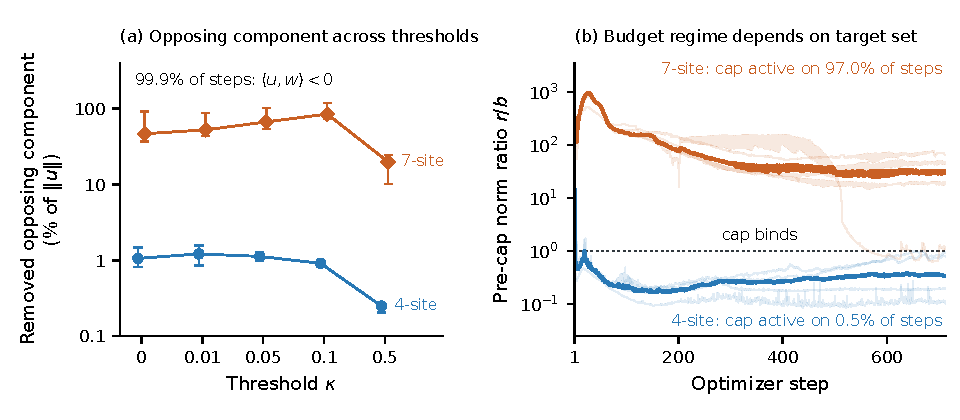
\includegraphics[width=\linewidth]{figures/02-14m-ol1-geometry.pdf}
\caption{\textbf{Pressure targets change OL1 geometry and cap activity.}
(a) Median $100\rho_{\mathrm{opp}}$ over 712 steps per condition; whiskers
are the 25th--75th percentiles. (b) Pre-cap norm ratio at $\lambda=b=1$;
faint curves are five thresholds per target set, thick curves their per-step
median. Cap-active fractions use the implemented scale $s<1$. Geometry is
measured before group learning rates and decoupled weight decay; it does
not guarantee task-loss preservation (Appendix~\ref{app:pressure}).}
\label{fig:ol1-geometry}
\end{figure}

\subsection{Broader threshold placement without pressure}
\label{sec:qkv-thresholding-results}

Pressure-free four-/seven-site comparisons keep $\kappa$ matched while
adding Q/K/V thresholds (Table~\ref{tab:qkv-thresholding}). At zero threshold
these added nonlinearities are identities, and the endpoints nearly
coincide. At $\kappa=0.5$, broader thresholding adds $5.17$ pp for
$+0.043$ loss. This control separates threshold placement from the
complete-recipe pressure interaction.

\begin{table}[htbp]
\centering\small
\caption{\textbf{Four- versus seven-site thresholds without pressure.}
A4 targets $a,m,h,z$; A7 additionally targets $q,k,v$. Values are raw
matched endpoints, not pressure effects.}
\label{tab:qkv-thresholding}
% Source observation: analyses/021-2026-09-10-training-results-figures/observations/O004-qkv-thresholding.md
% Retained evidence: analyses/018-2026-09-08-results-materials/figure_data.json
% Five matched 14M A4/A7 endpoints without pressure; loss and pooled integer-count sparsity use the same full-validation pass.
\begin{tabular}{@{}rrrrr@{}}
\toprule
$\kappa$ & A4 loss & A7 loss & A4 $\Smodel$ (\%) & A7 $\Smodel$ (\%) \\
\midrule
0 & 5.4705 & 5.4684 & 7.212 & 7.218 \\
0.01 & 5.4665 & 5.4588 & 7.414 & 7.618 \\
0.05 & 5.4341 & 5.4379 & 8.206 & 9.127 \\
0.1 & 5.4197 & 5.4287 & 8.953 & 10.425 \\
\textbf{0.5} & \textbf{5.6597} & \textbf{5.7029} & \textbf{10.216} & \textbf{15.387} \\
\bottomrule
\end{tabular}

\end{table}

\subsection{Local sparsity does not determine model-wide sparsity}
\label{sec:activation-reshaping}

At $\kappa=0.5$, expanding four-site OL1 to seven sites reduces exact zeros
at the \textbf{FFN-up input $m$ from 96.77\% to 68.70\%}, whereas the FFN
hidden activation $h$ changes only from 99.94\% to 99.88\%
(Figure~\ref{fig:activation-reshaping}). These are measured per-site counts,
not estimates from rounded operation contributions. Pooling $h,m$ would
weight them 80:20 and obscure the distinction. Layer-level counts appear
in Appendix Figure~\ref{fig:site-zero-heatmap}.

Despite fewer zeros at $m$, seven-site OL1 reaches $27.48\%$ model-wide
sparsity versus $12.71\%$ for four-site, with lower loss (5.8294 versus
6.0380). The decomposition explains why: $QK+PV$ contribute $16.77$ pp
versus $0.06$ pp, outweighing smaller projection contributions. FFN-up
contribution falls from $4.139$ to $2.939$ pp, while FFN-down remains
approximately $4.27$ pp. The pressure-free bars show the corresponding
placement comparison without OL1.

Four-site OL1's Q/K/V density concentrates near zero, yet only $0.22\%$
of these activations are exactly zero, versus $95.60\%$ with seven-site
OL1. Since four-site recipes do not directly target Q/K/V, their difference
from the dense reference is a \emph{nonlocal response of the trained
network}. It does not isolate pressure, thresholding, or their interaction.
Likewise, the FFN-up change may reflect target reweighting, cap behavior,
or representation adaptation; the present controls do not distinguish them.

\begin{figure}[tbp]
\centering
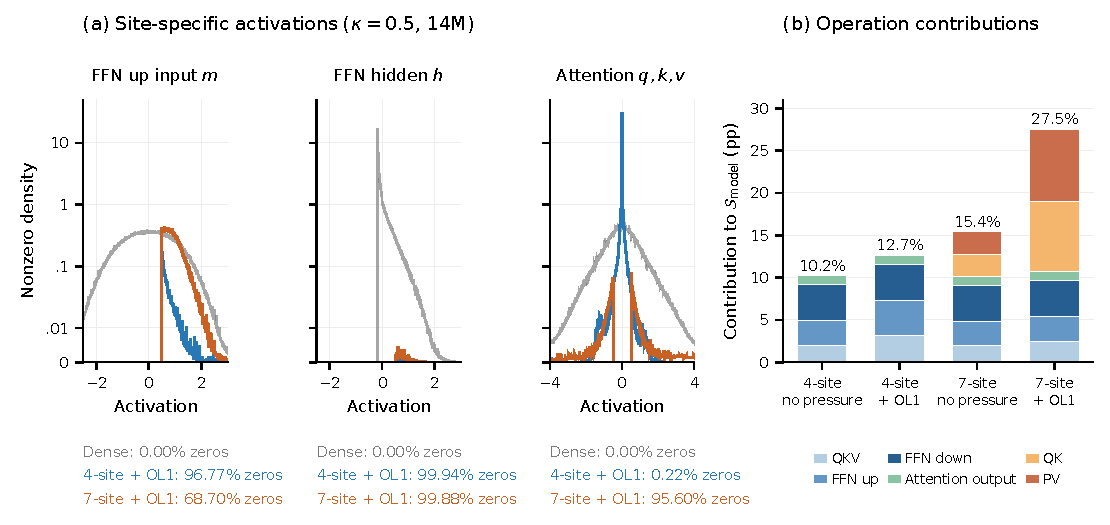
\includegraphics[width=\linewidth]{figures/review/04-site-distributions.pdf}
\caption{\textbf{Site-specific zeros and operation-weighted consequences.}
(a) Nonzero densities at $m$, $h$, and pooled Q/K/V, separately, for the
dense reference and four-/seven-site OL1 at $\kappa=0.5$; exact-zero
percentages appear below. Counts pool validation sequences and layers;
density divides by all elements and bin width, without renormalizing the
nonzero mass. (b) Four-/seven-site endpoints with and without OL1 at
$\kappa=0.5$. Stacks use the common full-model denominator, including the
dense vocabulary head. Bars measure zero-product opportunities, not time
savings. Pressure-free density measurements are unavailable; their bars
use the retained logical counters.}
\label{fig:activation-reshaping}
\end{figure}

\subsection{Cross-size recipe evaluation}
\label{sec:scale-results}

\textbf{At the largest tested threshold, $\kappa=0.5$, seven-site OL1 has
lower loss and greater $\Smodel$ than four-site OL1 at all three sizes}
(Figure~\ref{fig:scale-transfer}). At $\kappa=0$, four-site is better on
both axes at 14M and 70M, but seven-site is better at 410M. This is recurrence
of one complete-recipe ordering, not transfer of the full threshold response.
The larger cohorts lack pressure-free multisite controls; exact contrasts
are in Appendix Table~\ref{tab:scale-pairs-full}.

Seven-site reach rises from $29.95\%$ to $49.42\%$ to $87.25\%$, partly
because the dense vocabulary head contributes a smaller share as width and
depth grow. The $\kappa=0.5$ endpoints reach $27.48\%$, $40.60\%$, and
$80.62\%$ $\Smodel$: 91.8\%, 82.2\%, and 92.4\% of these references.
Their dense-relative loss penalties are $+0.6208$, $+1.1162$, and $+0.5732$
(perplexity factors $1.86$, $3.05$, and $1.77$). Thus the larger raw
sparsity at 70M does not imply an improved quality cost or reference ratio.
The seven-site coverage formula in Appendix~\ref{app:architecture-counts}
makes its architecture-and-workload dependence explicit.

Dense losses themselves are non-monotonic: 5.2086, 4.0998, and 4.5475.
The fixed token budget supplies 106.14, 21.20, and 3.68 tokens per parameter;
410M also has a lower peak learning rate. Its different realized optimization
regime is not evidence of premature convergence or failure to converge
(Appendix Figure~\ref{fig:a0-optimization}). These experiments test
within-size recipe relationships rather than a quality scaling law.

\begin{figure}[tbp]
\centering
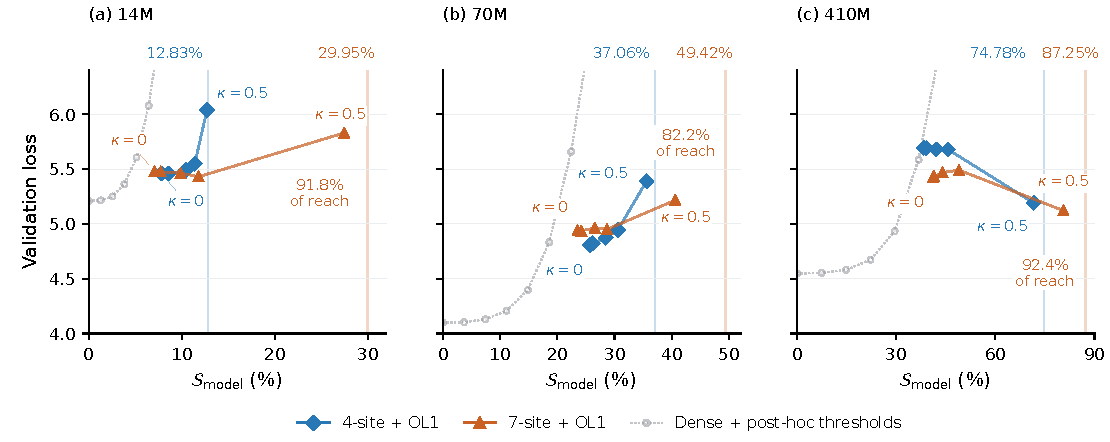
\includegraphics[width=\linewidth]{figures/review/05-cross-size.pdf}
\caption{\textbf{The $\kappa=0.5$ complete-recipe ordering recurs across sizes.}
Absolute loss versus $\Smodel$ for independently trained four-/seven-site
OL1 conditions; points use $\kappa\in\{0,0.01,0.05,0.1,0.5\}$.
Gray dotted curves apply four-site post-hoc magnitude thresholding to the
dense references. Vertical guides mark selected-site reach for full-sequence,
full-vocabulary inference; endpoint annotations are reference ratios.
Axes share the loss range but use size-specific sparsity ranges. Lines
connect evaluated settings; complete post-hoc paths are in
Appendix~\ref{app:clipping-results}.}
\label{fig:scale-transfer}
\end{figure}

% Evidence: Analysis024 observations/034-operation-latency-manuscript.md;
% Run037 observations/001-operation-latency.md and results/conditional-effects-audit.json.
% Table generator: Analysis024/25_build_operation_latency_table.py.
% a/m port evidence: Analysis024 observations/035-am-load-avoidance-port.md;
% Run039 observations/001-am-port-verdict.md, results/am-load-avoidance.json
% and results/mechanism.json; reducers: Run039/07_reduce.py and 12_mechanism.py.
% Mechanism: Run028 candidates/k049/joint.cu, k042/projection.cu,
% k035/sparse_gemm.h and k035/flash_fwd_kernel.h; Run029 implementation audit.
\subsection{When model-wide sparsity translates to speedup}
\label{sec:activation-reshaping}
\label{sec:kernel-autoresearch}

Sparsity reduces latency when avoided work exceeds the cost of detecting and
skipping zeros. At $h,z$, our kernel checks $8\times16$ activation groups
before loading their weights: empty groups avoid both weight reads and matrix
multiplications. At $a,m$, the $16\times16$ checks occur after both operands
are loaded, so skipping saves only arithmetic.
A follow-up test supports this choice: applying the $h/z$ strategy separately
at $a$ and $m$ increased full-model latency by $17.2\%$ and $27.4\%$ on
14M $T_7/P_{\mathrm{all}}$ at $\kappa=0.5$, with unchanged outputs.
Only $11.12\%$ of $a$'s $8\times16$ tiles were empty, and none at $m$, so
most groups still required matrix multiplication. Padding eight real rows to
sixteen-row matrix instructions increased issued instructions by $1.90\times$
at $a$ and $2\times$ at $m$. At $h/z$, most rows instead have at most two
nonzero activations, making the cheaper scalar path useful much more often.

Attention follows FlashAttention's tiled sequence \citep{dao2022flashattention}:
load $Q,K$, compute scores, apply masking and softmax, then multiply
probabilities by $V$. Our checks occur after operand loads; skipping an empty
tile's multiplication cannot recover those reads. Softmax still runs and
turns zero scores into nonzero probabilities, so $Q/K$ sparsity does not
automatically propagate to $PV$. Zeros in $V$ remain usable; sparsifying the
probabilities is a further opportunity, untested here.

We isolate each path's effect at 14M by disabling it while holding weights,
gates and all other skipping paths fixed (Table~\ref{tab:kernel-mechanisms}).
\emph{Bypass} counts skipped matrix instructions divided by issued plus
skipped instructions; it does not measure the fraction of runtime saved.

\begin{table}[!htbp]
\centering\small
\caption{\textbf{Conditional latency savings: 14M $T_7/P_{\mathrm{all}}$, $\kappa=0.5$.}
Times are per 2,048-token sequence on RTX\,5090 (BF16, batch one).
Saved time is full-model latency with one skipping path off minus latency
with all paths on; positive values indicate a benefit.
Brackets give [minimum, maximum] savings across all off/on pairs of three
independent timing runs per mode, not confidence intervals.
Each run reports the geometric mean over 64 sequences and seven passes.
Effects are not additive.}
\label{tab:kernel-mechanisms}
% Generated by Analysis024/25_build_operation_latency_table.py.
\begin{tabular}{@{}lrrr@{}}
\toprule
Operation & Bypass (\%) & Saved time ($\mu$s) & Process span ($\mu$s) \\
\midrule
$a$: QKV projection & 8.4 & $-1.6$ & $[-6.0, +3.8]$ \\
$m$: FFN-up & 0.0 & $-2.4$ & $[-5.1, +2.7]$ \\
$h$: FFN-down & 94.5 & $+150.1$ & $[+145.4, +154.4]$ \\
$z$: attention-output projection & 99.6 & $+29.0$ & $[+23.7, +35.7]$ \\
$q,k$: $QK$ scores & 58.0 & $-2.9$ & $[-7.3, +1.1]$ \\
$v$: $PV$ product & 67.2 & $-6.2$ & $[-9.0, -2.2]$ \\
\bottomrule
\end{tabular}

\end{table}

The clear savings come from $h$ ($150\,\mu$s) and $z$ ($29\,\mu$s).
Individual $a,m,QK$ effects remain unresolved against process variation,
whereas $PV$ skipping adds latency. Enabling $QK/PV$ skipping together raises
full-model latency from 0.514 to 0.521\,ms despite substantial bypass.
Thus, for this checkpoint and implementation, attention's arithmetic savings
do not offset its overhead, while $h/z$ benefit from avoiding weight reads
as well as computation.

\FloatBarrier

